\section{Event Selection}%
\label{sec:event_selection}

Events consistent with the signature of $\bbbar\lephad$ and $\bbbar\hadhad$
final states are selected. A loose event selection is applied that is largely
determined by the triggers employed in this search. The discrimination of signal
and background events is not the primary goal of the event selection but rather
of a multivariate analysis that is introduced in
\Cref{sec:multivariate_analysis}.
% In addition, control and validation regions are defined for the purpose of
% estimating backgrounds or validating background estimates.

All events considered in this analysis are required to have a reconstructed
primary vertex. Moreover, events containing one or more jets that are classified
as originating from non-collision backgrounds or calorimeter noise according to
a loose jet cleaning working point~\cite{ATLAS-CONF-2015-029} are rejected.

% Events considered for further analysis are required to fulfil basic
% quality criteria independent of the analysis channel:
% \begin{itemize}
%   % GRL + basic checks

%   % eventInfoIn->errorState(xAOD::EventInfo::EventFlagSubDet::Tile) == xAOD::EventInfo::Error
%   % Problems in tile calorimeter (``tile corrupted events''')
%   %
%   % eventInfoIn->errorState(xAOD::EventInfo::EventFlagSubDet::LAr) == xAOD::EventInfo::Error
%   % LAr noise bursts
%   %
%   % eventInfoIn->errorState(xAOD::EventInfo::EventFlagSubDet::SCT) == xAOD::EventInfo::Error
%   % SCT corrupted events (``recovery period after single event upset''')
%   %
%   % eventInfoIn->isEventFlagBitSet(xAOD::EventInfo::Core,18
%   % Event info missing after TTC restart
% \item All events are required to fulfil the data quality criteria by the ATLAS
%   collaboration~\cite{DAPR-2018-01} requiring stable beams at the LHC and a
%   fully operational detector.

%   % Has vertex
% \item The event is required to have a primary vertex.

%   % No fake jets
%   % DFCommonJets_eventClean_LooseBad
% \item Events containing one or more jets that are classified as originating
%   from non-collision backgrounds or calorimeter noise according to a
%   \emph{loose} jet cleaning~\cite{ATLAS-CONF-2015-029} working point are
%   rejected.
% \end{itemize}

The search is divided into different channels depending on the decay mode of the
\tauleptonC pair and the type of trigger that selected an event. The \lephad
channel targets semi-leptonic decay modes using single-lepton triggers (SLTs)
and lepton-plus-\tauhadvis triggers (LTTs). Each trigger defines a corresponding
sub-channel referred to as the \lephad SLT and \lephad LTT channel,
respectively. The \hadhad channel selects events with two \tauhadvis candidates
using single-\tauhadvis triggers (STTs) and di-\tauhadvis triggers (DTTs).
Events selected by STTs and DTTs are combined into a single channel.
% While different types of triggers are used in the \hadhad channel, the
% statistical analysis will not distinguish between events selected by STTs and
% DTTs.

% While different types of triggers are used in this channel, the later
% statistical analysis will not distinguish between events selected by STTs and
% DTTs, thus the \hadhad final state is treated as a single analysis channel. In
% some cases, for example for the background estimation, it will be required to
% distinguish between both trigger categories. Cases where this applies will be
% indicated explicitly.

Orthogonality between the \lephad and \hadhad channel is ensured by selections
on the number of electrons, muons, and \tauhadvis. In the \hadhad channel,
events are required to have exactly two \tauhadvis and events with electrons or
muons are rejected. In the \lephad channels, events are required to have exactly
one \tauhadvis and exactly one electron or muon. Additionally, electrons (muons)
are required to pass the tight (medium) identification working point to reduce
backgrounds with non-prompt leptons or jets misidentified as electrons (muons).

Electrons, muons, and \tauhadvis have to be geometrically matched to the
corresponding object at the HLT that fulfilled the criteria of the trigger that
selected the event.
% according to the trigger that selected the event.
This requirement is referred to as \emph{trigger-matching}. Trigger-dependent
\pT~thresholds are applied to electrons, muons, and \tauhadvis to ensure that
the triggers operate in regimes in which they are well-calibrated. The
\pT~thresholds of SLTs and STTs increased with increasing instantaneous
luminosity of the LHC during Run~2. For LTTs and DTTs, the \pT~thresholds on
electrons, muons, and \tauhadvis remained constant during Run~2, the
trigger-rates were instead limited by requiring additional jets at the L1
trigger.

% The inclusion of the \lephad LTT channel allows to select events with
% electrons or muons with transverse momenta below the SLT \pT~threshold by
% requiring an additional \tauhadvis at trigger-level. Orthogonality between the
% \lephad SLT and LTT channel is ensured by only considering events with lepton
% \pT below the SLT \pT~threshold for the LTT channel.

An overview of the signal region (SR) event selection is given in
\Cref{tab:event_selection}. A more detailed description of the \hadhad channel
trigger selection is given in \Cref{sec:hadhad_trigger_selection}. Further
selections applied at event-level to define the SRs are discussed in
\Cref{sec:sr_and_cr_selection}.

\begin{table}[htbp]
  \centering

  \caption[SR event selection for the \hadhad, \lephad SLT, and \lephad LTT
  channel.]{SR event selection for the \hadhad, \lephad SLT, and \lephad LTT
    channel. Trigger-dependent thresholds are applied to the \pT of electrons,
    muons, and \tauhadvis. Where applicable, the range of these thresholds is
    listed. Selections applied to \pT sub-leading objects are given in
    parenthesis. The trigger-dependent selections applied to \tauhadvis and jets
    in the \hadhad channel are described in
    \Cref{sec:hadhad_trigger_selection}. Forward jets are not used for event
    selection purposes. The table is adapted from Ref.~\cite{HDBS-2018-40}.}%
  \label{tab:event_selection}

  \resizebox{\textwidth}{!}{
    {
  \newcolumntype{C}[1]{>{\centering\let\newline\\\arraybackslash\hspace{0pt}}m{#1}}
  \small

  \begin{tabular}{C{0.225\textwidth}C{0.225\textwidth}C{0.225\textwidth}C{0.225\textwidth}}
    \toprule
    \multicolumn{2}{c}{\textbf{\hadhad channel}} & \multicolumn{2}{c}{\textbf{\lephad channels}} \\[0.5em]
    \textbf{STT} & \textbf{DTT} & \textbf{SLT} & \textbf{LTT} \\
    \midrule
    \multicolumn{4}{c}{\textbf{$e$ / $\mu$ selections}} \\
    \midrule
    \multicolumn{2}{c}{No loose $e$ or $\mu$} & \multicolumn{2}{c}{Exactly one loose $e$ or one loose $\mu$} \\[0.5em]
                                                 && \multicolumn{2}{c}{$e$ passes tight ID or} \\
                                                 && \multicolumn{2}{c}{$\mu$ passes medium ID and $|\eta| < 2.5$} \\[0.5em]
                                                 && $\pT(e) > 25\text{--}\SI{27}{\GeV}$ & $\pT(e) > \SI{18}{\GeV}$ \\
                                                 && $\pT(\mu) > 21\text{--}\SI{27}{\GeV}$ & $\pT(\mu) > \SI{15}{\GeV}$ \\[0.5em]
                                                 &&& Lepton \pT below SLT threshold \\
    \midrule
    \multicolumn{4}{c}{\textbf{\tauhadvis selections}} \\
    \midrule
    \multicolumn{2}{c}{Exactly two \tauhadvis} & \multicolumn{2}{c}{Exactly one \tauhadvis} \\[0.5em]
                                                 && \multicolumn{2}{c}{$|\eta| < 2.3$} \\[0.5em]
    $\pT > 100\text{--}180 \, (25)\,\si{\GeV}$ & $\pT > 40 \, (30)\,\si{\GeV}$ & & $\pT > \SI{30}{\GeV}$ \\
    \midrule
    \multicolumn{4}{c}{\textbf{Central jet selections ($|\eta| < 2.5$)}} \\
    \midrule
    \multicolumn{4}{c}{$\geq 2$ jets}\\[0.5em]
    $\geq 1$ jet with $\pT > \SI{45}{\GeV}$ & Trigger-dependent & $\geq 1$ jet with $\pT > \SI{45}{\GeV}$ & Trigger-dependent \\
    \midrule
    \multicolumn{4}{c}{\textbf{Event-level selections}} \\
    \midrule
    \multicolumn{4}{c}{Event is selected by a trigger and trigger requirements are fulfilled} \\[0.25em]
    \multicolumn{4}{c}{Exactly 2 $b$-tagged jets} \\[0.25em]
    \multicolumn{4}{c}{Opposite sign electric charge between \tauhadvis and $e$ / $\mu$ / \tauhadvis} \\[0.25em]
    \multicolumn{4}{c}{$\mMMC > \SI{60}{\GeV}$} \\[0.25em]
                                                 && \multicolumn{2}{c}{$\mBB < \SI{150}{\GeV}$} \\
    \bottomrule
  \end{tabular}
}

%%% Local Variables:
%%% mode: latex
%%% TeX-master: "../phd_thesis"
%%% End:

  }
\end{table}


\subsection{Trigger Selection in the \hadhad Channel}%
\label{sec:trigger}%
\label{sec:hadhad_trigger_selection}

% This section describes the trigger selection of the \hadhad channel.
The triggers used in the \hadhad channel depend on the data-taking period due to
the changing instantaneous luminosity and introduction of new trigger algorithms
during Run~2 of the LHC.
% Due to the changing instantaneous luminosity during Run~2 of the LHC, the
% triggers used in this analysis depend on the data-taking period.
A list of triggers considered in this search is given in
\Cref{tab:triggers_hadhad}. Further explanations of the items in the table are
given in the remainder of this section.

\begin{sidewaystable}[p]
  \centering

  \caption[Summary of STTs and DTTs used in the \hadhad channel.]{Summary of
    STTs and DTTs used in the \hadhad channel. The trigger naming scheme follows
    the conventions by the ATLAS collaboration. An explanation of these triggers
    is given in the main body. The ``offline event selection'' column summarises
    selections applied to \tauhadvis and jets during the offline event
    reconstruction to ensure that the triggers operate close to their
    trigger-efficiency plateau. These requirements are specified in terms of the
    \pT leading or sub-leading \tauhadvis ($\tau_0$ or $\tau_1$) and the \pT
    leading or sub-leading central jet ($\text{j}_0$ or $\text{j}_1$). All
    events selected by DTTs have to fulfil $\pT(\tau_0) > \SI{40}{\GeV}$ and
    $\pT(\tau_1) > \SI{30}{\GeV}$ (omitted in the table). The last column
    specifies the data-taking period in which a trigger was used.}

  % Requirements on \tauhadvis and jets from offline event reconstruction
  % (offline requirements) are imposed. These requirements are specified in
  % terms of the leading or sub-leading \tauhadvis ($\tau_0$ or $\tau_1$) or the
  % leading or sub-leading central jet ($\text{j}_0$ or $\text{j}_1$). For all
  % events selected by DTT, \tauhadvis have to fulfil
  % $\pT(\tau_0) > \SI{40}{\GeV}$ and $\pT(\tau_1) > \SI{30}{\GeV}$. The
  % data-taking periods where triggers were used are given in the last column.


  % \pT~\thresholds on \tauhadvis at the HLT are denoted by \texttt{tauX}, where
  % \texttt{X} is the threshold in \si{GeV}. The differences between HLT chains
  % are explained in the main body. The \ET and isolation requirements on
  % \tauhadvis at the L1~trigger are denoted by \texttt{nTAUx}(\texttt{I} or
  % \texttt{IM}), where \texttt{x} is the \ET~threshold in \si{\GeV}, \texttt{I}
  % and \texttt{IM} are isolation requirements, and \texttt{n} is the number of
  % \tauhadvis fulfilling these conditions. Similarly, jets at the L1 trigger
  % are denoted by \texttt{nJx}(\texttt{.0ETA23}), where \texttt{x} is the jet
  % \ET~threshold in \si{\GeV}, the suffix \texttt{.0ETA23} indicates a
  % requirement of $|\eta| < 2.3$ on jets, and \texttt{n} is the number of jets
  % passing these selections.

  % in the main body. The \ET and isolation requirements on \tauhadvis at the L1
  % trigger are denoted by \texttt{xTAUy}(\texttt{I}/\texttt{IM}) with
  % \texttt{y} being the \ET~threshold in \si{\GeV}, \texttt{I}/\texttt{IM}
  % being isolation requirements, and \texttt{x} being the number of \tauhadvis
  % fulfilling these conditions. Similarly, jets at the L1 trigger are denoted
  % by \texttt{xJy}(\texttt{.0ETA23}), where \texttt{y} is the jet \ET~threshold
  % in \si{\GeV}, the suffix \texttt{.0ETA23} indicating a requirement of
  % $|\eta| < 2.3$ on jets, and \texttt{x} is the number of jets that pass these
  % conditions.  Unless a trigger is based on the L1 topological trigger
  % system~\cite{TRIG-2019-02} (L1Topo), here chains using the
  % \texttt{DR-TAU20ITAU12I-J25} seed, no disambiguation between objects at L1
  % is performed such that one \texttt{TAU20IM} also ensures at least one count
  % of \texttt{TAU12IM}, \texttt{J20}, and \texttt{J12}. For chains based on
  % L1Topo, disambiguation is performed and additionally \tauhadvis at L1 are
  % required to fulfil
  % $\Delta R(\tau_0^{\text{L1}}, \tau_1^{\text{L1}}) \leq 2.8$.  Requirements
  % on \tauhadvis and jets from offline event reconstruction (offline
  % requirements) are imposed. These requirements are specified in terms of the
  % leading or sub-leading \tauhadvis ($\tau_0$ or $\tau_1$) or the leading or
  % sub-leading central jet ($\text{j}_0$ or $\text{j}_1$). For all events
  % selected by DTT, \tauhadvis have to fulfil $\pT(\tau_0) > \SI{40}{\GeV}$ and
  % $\pT(\tau_1) > \SI{30}{\GeV}$. The data-taking periods where triggers were
  % used are given in the last column.}%
  \label{tab:triggers_hadhad}

  \resizebox{\textwidth}{!}{
    \begin{tabular}{lllll}
  \toprule
  \textbf{HLT chain} & \textbf{} & \textbf{L1 trigger} & \textbf{Offline event selection} & \textbf{Period} \\
  \midrule
  \multicolumn{5}{l}{Single-\tauhadvis triggers} \\
  \midrule
  \texttt{tau80} & \texttt{medium1\_tracktwo} & \texttt{TAU60} & $\pT(\tau_0) > \SI{100}{\GeV}$ & 15--16 A \\
  \texttt{tau125} & \texttt{medium1\_tracktwo} & \texttt{TAU60} & $\pT(\tau_0) > \SI{140}{\GeV}$ & 16 B--16 D3\\
  \texttt{tau160} & \texttt{medium1\_tracktwo} & \texttt{TAU60} & $\pT(\tau_0) > \SI{180}{\GeV}$ & 16 D4--17 B4\\
  \texttt{tau160} & \texttt{medium1\_tracktwo} & \texttt{TAU100} & $\pT(\tau_0) > \SI{180}{\GeV}$ & 17 B5--17 end\\
  \texttt{tau160} & \texttt{medium1\_tracktwoEF} & \texttt{TAU100} & $\pT(\tau_0) > \SI{180}{\GeV}$ & 18-- \\
  \texttt{tau160} & \texttt{mediumRNN\_tracktwoMVA} & \texttt{TAU100} & $\pT(\tau_0) > \SI{180}{\GeV}$ & 18 K-- \\
  \midrule
  \multicolumn{5}{l}{Di-\tauhadvis triggers} \\
  \midrule
  \texttt{tau35} + \texttt{tau25} & \texttt{medium1\_tracktwo} & \texttt{TAU20IM\_2TAU12IM} & $\pT(\text{j}_0) > \SI{80}{\GeV}$ & 15--15 end \\
  \texttt{tau35} + \texttt{tau25} & \texttt{medium1\_tracktwo} & \texttt{TAU20IM\_2TAU12IM\_J25\_2J20\_3J12} & $\pT(\text{j}_0) > \SI{80}{\GeV}$ & 16--17 B4 \\
  \texttt{tau35} + \texttt{tau25} & \texttt{medium1\_tracktwo} & \texttt{TAU20IM\_2TAU12IM\_4J12} & $\pT(\text{j}_1) > \SI{45}{\GeV}$ & 17--17 end \\
  \texttt{tau35} + \texttt{tau25} & \texttt{medium1\_tracktwo} & \texttt{DR-TAU20ITAU12I-J25} & $\pT(\text{j}_0) > \SI{80}{\GeV}$, $\Delta R(\tau_0, \tau_1) < 2.5$ & 17 B5--17 end \\
  \texttt{tau35} + \texttt{tau25} & \texttt{medium1\_tracktwoEF} & \texttt{TAU20IM\_2TAU12IM\_4J12.0ETA23} & $\pT(\text{j}_1) > \SI{45}{\GeV}$ & 18-- \\
  \texttt{tau35} + \texttt{tau25} & \texttt{medium1\_tracktwoEF} & \texttt{DR-TAU20ITAU12I-J25} & $\pT(\text{j}_0) > \SI{80}{\GeV}$, $\Delta R(\tau_0, \tau_1) < 2.5$ & 18-- \\
  \texttt{tau35} + \texttt{tau25} & \texttt{mediumRNN\_tracktwoMVA} & \texttt{TAU20IM\_2TAU12IM\_4J12.0ETA23} & $\pT(\text{j}_1) > \SI{45}{\GeV}$ & 18 K-- \\
  \texttt{tau35} + \texttt{tau25} & \texttt{mediumRNN\_tracktwoMVA} & \texttt{DR-TAU20ITAU12I-J25} & $\pT(\text{j}_0) > \SI{80}{\GeV}$, $\Delta R(\tau_0, \tau_1) < 2.5$ & 18 K-- \\
  \bottomrule
\end{tabular}

%%% Local Variables:
%%% mode: latex
%%% TeX-master: "../phd_thesis"
%%% End:

  }
\end{sidewaystable}

As Run~2 of the LHC progressed, several improvements were made to the HLT
algorithms used in \tauhadvis-triggers. Consequently, three different HLT chains
are used in this analysis, the differences between them are described in the
following:
\begin{description}

\item[\texttt{medium1\_tracktwo}] This chain is the primary HLT chain for
  \tauhadvis-triggers in the data-taking period from 2015 to
  2017~\cite{ATL-DAQ-PUB-2016-001,ATL-DAQ-PUB-2017-001,ATL-DAQ-PUB-2018-002}. A
  brief summary based on Ref.~\cite{ATLAS-CONF-2017-061} is given hereafter.

  First, a purely calorimeter-based reconstruction of the \tauhadvis candidate
  is performed in the region of interest (ROI) provided by the L1 trigger. The
  topo-cluster algorithm is applied to the calorimeter cells in the ROI and the
  resulting topo-clusters are calibrated using the local hadronic
  calibration. The energy of \tauhadvis candidates is determined from clusters
  in a core region ($\Delta R < 0.2$) around the barycentre of topo-cluster
  energy in the ROI. Subsequently, a \tauhadvis-specific energy calibration is
  applied.
  % subsequently applying a \tauhadvis-specific calibration which is a function
  % of \tauhadvis candidate \pT, $\eta$, and pile-up conditions.
  The HLT threshold on the \pT of \tauhadvis candidates is applied after these
  steps.

  Second, a two-stage tracking approach using \emph{fast tracking}, instead of
  the more time-consuming \emph{precision tracking} algorithm used during
  offline event reconstruction (cf.~\Cref{sec:tracking_and_vertexing}) and at
  later stages of the trigger, is
  employed~\cite{TRIG-2016-01,ATLAS-CONF-2017-061,TRIG-2019-03}.
  % instead of the more time-consuming offline track reconstruction algorithms
  % (\emph{precision tracking}), is
  % employed~\cite{TRIG-2016-01,ATLAS-CONF-2017-061,TRIG-2019-03}.
  The first stage performs tracking in a narrow region surrounding the
  \tauhadvis candidate close to the calorimeters but extended over a large
  section of the beamline. The \pT-leading track resulting from this stage is
  used to narrow down the search space along the beamline by only considering
  the beamline section within $|\Delta z| < \SI{10}{\milli\metre}$ of this track
  for the second stage of tracking, thus allowing for an expansion of the search region
  close to the calorimeters. After the second
  stage of tracking, core and isolation tracks are defined according to the
  conditions $\Delta R(\text{track}, \tauhadvis) < 0.2$ and
  $0.2 < \Delta R(\text{track}, \tauhadvis) < 0.4$, respectively. Subsequently,
  track multiplicity selections are applied by requiring \tauhadvis candidates
  to have one to three core tracks and at most one isolation track.

  Lastly, a \tauhadvis selection similar to the offline \tauhadvis selection is
  performed. The tracks resulting from the two-stage tracking are used as seeds
  for precision tracking. The precision tracks are then used to calculate
  discriminating variables used for \tauid. A BDT-based \tauid algorithm
  % , similar to its counterpart from the offline \tauhadvis reconstruction,
  is applied and \tauhadvis are required to pass the \emph{medium} working
  point.\footnote{The medium working point of the HLT \tauid applies less
    stringent requirements than the loose working point of the RNN-based \tauid
    algorithm applied during offline event reconstruction.}

\item[\texttt{medium1\_tracktwoEF}]
  % The precision tracks are also called EF tracks, while fast tracks
  % are called FTF tracks.
  This chain was introduced for data-taking in 2018~\cite{ATL-DAQ-PUB-2019-001}
  and differs from the previous item by delaying the track multiplicity
  selections to a later stage of the HLT chain. Instead of counting tracks from
  the two-stage fast track finding, the track multiplicities are defined using
  precision tracks. This change circumvents a reduction in efficiency for
  3-prong \tauhadvis in high pile-up conditions due to the fast track finding
  being more susceptible to fake tracks~\cite{ATL-DAQ-PUB-2019-001}.

\item[\texttt{mediumRNN\_tracktwoMVA}] This chain started operation in period K
  of 2018 data-taking~\cite{ATL-DAQ-PUB-2019-001}. The integrated luminosity
  from period K to the end of Run~2 corresponds to about
  \SI{37}{\per\femto\barn}. Several changes were implemented on top of the
  \texttt{medium1\_tracktwoEF} chain.

  First, the \tauhadvis energy calibrations as part of the calorimeter-based
  \tauhadvis reconstruction are replaced by multivariate methods. Second, the
  HLT \tauid is replaced by a method based on the RNN \tauid algorithm
  introduced in \Cref{sec:tauid}. The improved background rejection of this
  algorithm allowed relaxing the track multiplicity requirements from 1--3
  precision tracks to 0--3 precision tracks in the core region. Selecting
  \tauhadvis candidates without precision tracks in the core region recovers
  cases in which the fast track finding does not yield good quality seeds for
  the precision tracking. After the offline event reconstruction, a fraction of
  these events can be correctly reconstructed, thus improving the selection
  efficiency of the trigger.

  The \texttt{mediumRNN\_tracktwoMVA} HLT chain is intended to be used in
  conjunction with the \texttt{medium1\_tracktwoEF} chain by combining both
  using a logical \emph{or}. Calibrations for this combination are provided by
  the ATLAS collaboration.
\end{description}

% INCLUDE OR NOT INCLUDE???
%
% \begin{figure}[htbp]
%   \centering

%   \begin{subfigure}{.49\textwidth}
%     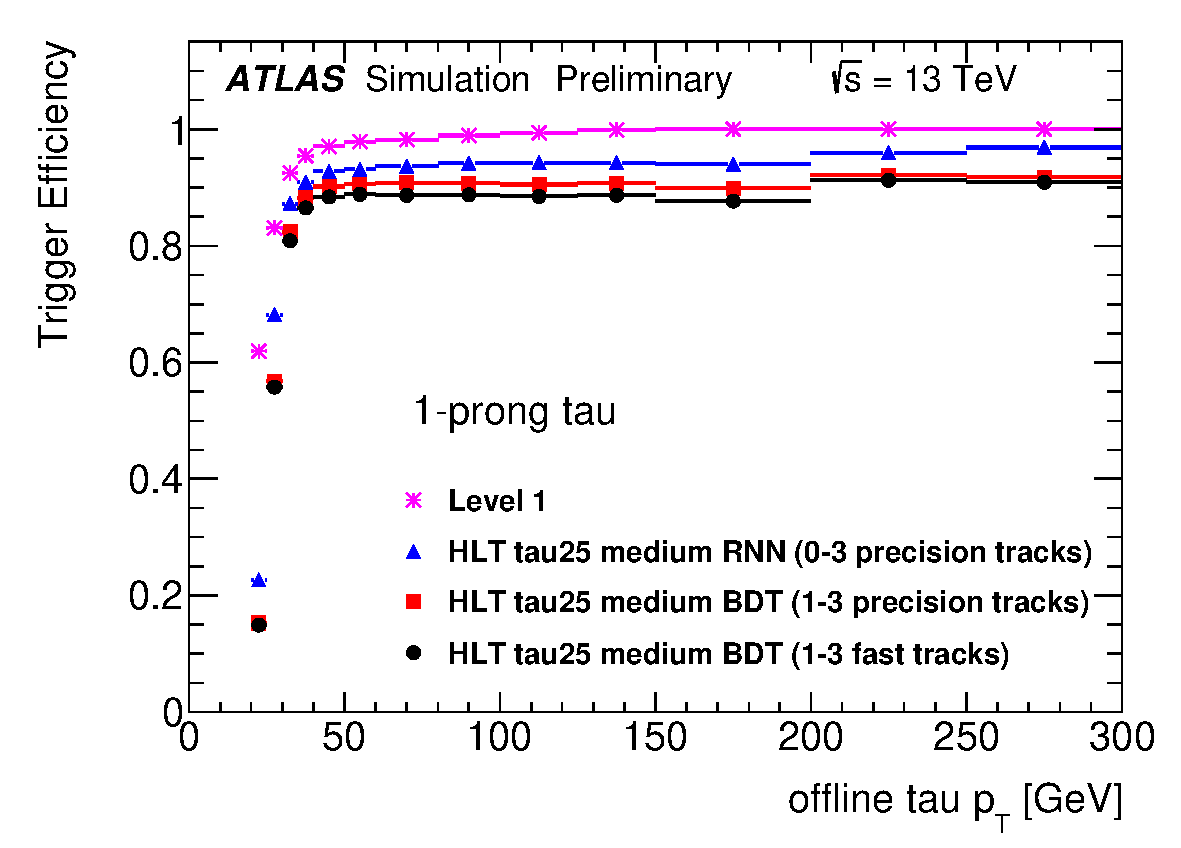
\includegraphics[width=\textwidth]{selection/trig_eff_1p}
%     \caption{$\Ntracks = 1$}
%   \end{subfigure}\hfill
%   \begin{subfigure}{.49\textwidth}
%     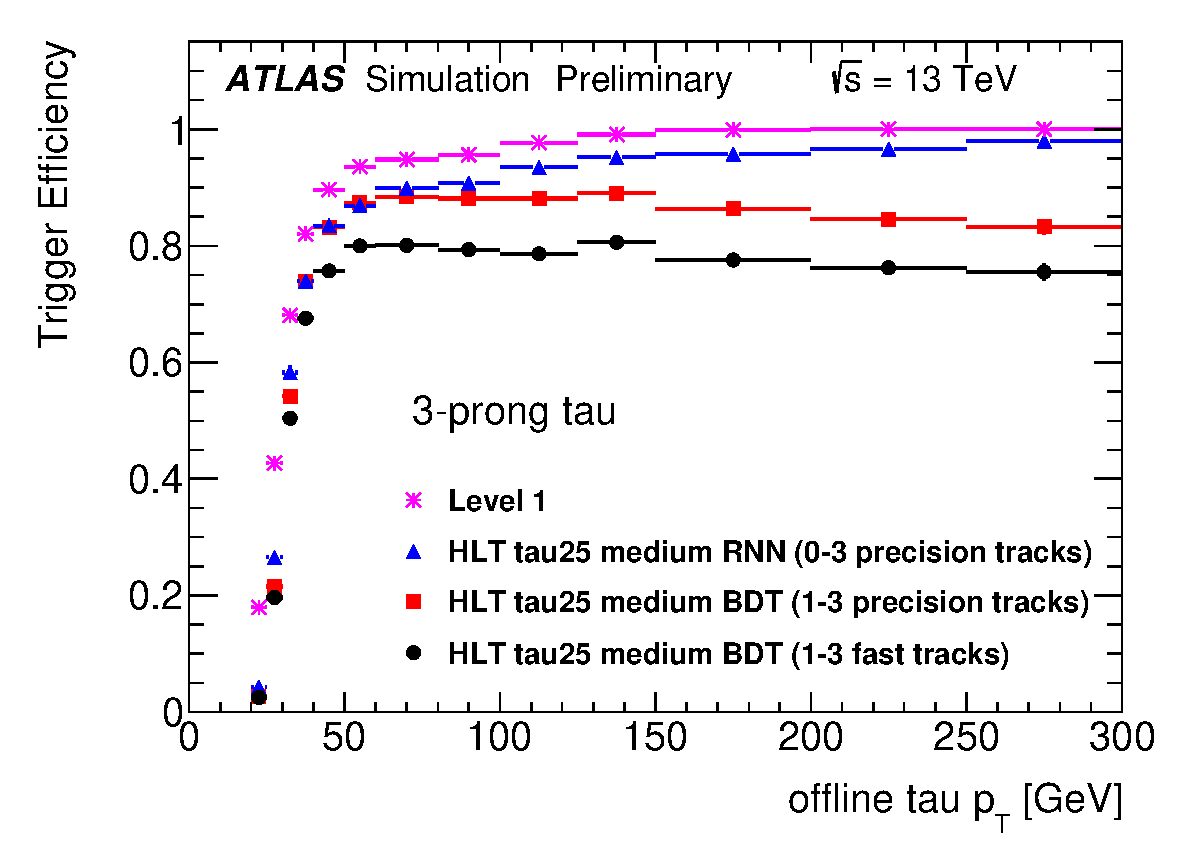
\includegraphics[width=\textwidth]{selection/trig_eff_3p}
%     \caption{$\Ntracks = 3$}
%   \end{subfigure}

%   \caption{Trigger efficiencies. The figures are taken from
%     Ref.~\cite{ATL-DAQ-PUB-2019-001}.}
%   \label{fig:trigger_efficiencies}
% \end{figure}

% Both single- and di-\tauhadvis triggers are used to select events of
% interest for the \hadhad channel. When an event fulfils both the STT
% and DTT criteria, precedence is given to the STT.

\subsubsection{STT Selection}

The STTs used in this analysis have varying \pT~thresholds applied to \tauhadvis
candidates depending on the data-taking period. At the HLT, these thresholds
range from \SI{80}{\GeV} to \SI{160}{\GeV}. An event is considered to pass the
STT selection if the following conditions are true: the event was selected by a
STT, it has at least one \tauhadvis candidate geometrically matched to a
\tauhadvis at the HLT ($\Delta R < 0.2$), and the \pT of the trigger-matched
\tauhadvis candidate exceeds the HLT \pT~threshold by \SIrange{15}{20}{\GeV}.
% The STT selection requires at least one \tauhadvis from the offline event
% reconstruction to be geometrically matched ($\Delta R < 0.2$) to a \tauhadvis
% at the HLT. Moreover, the \pT of the \tauhadvis has to exceed the
% \pT~threshold at the HLT by \SIrange{15}{20}{\GeV}.
The exact offline event selection requirements are given
in~\Cref{tab:triggers_hadhad}.

\subsubsection{DTT Selection}

The \tauhadvis \pT requirements of the DTTs used in this search remain unchanged
throughout Run~2 of the LHC. At the HLT, the \pT~thresholds on the leading and
sub-leading \tauhadvis candidate are \SI{35}{\GeV} and \SI{25}{\GeV},
respectively. Events are considered as possible DTT events if they fulfil the
following requirements: First, both \tauhadvis candidates from the offline event
reconstruction have to be trigger-matched. Second, the trigger-matched
\tauhadvis have to exceed the corresponding HLT \pT~threshold by at least
\SI{5}{\GeV}.

The primary limitations of DTTs arise at the L1~trigger, requiring changes in
L1~seeds as the instantaneous luminosity increased during Run~2
data-taking. This is reflected in the DTT trigger selection described in the
following:
\begin{description}

\item[2015 data-taking period] The DTT used in 2015
  (cf.~\Cref{tab:triggers_hadhad}) had no additional requirements beyond two
  isolated \tauhadvis at the L1 trigger. However, a requirement of
  $\pT > \SI{80}{\GeV}$ is applied to the \pT-leading central jet from the
  offline event reconstruction. This selection is not strictly necessary and is
  applied to unify the selection with the DTT used in 2016.
  % \footnote{The integrated luminosity collected in 2015 is small
  % (\SI{3.2}{\per\femto\barn}) compared to the full Run~2 \pp~collision
  % dataset thus motivating the use of a cut that is tighter than necessary in
  % favour of harmonising the selection between data-taking periods.}

\item[2016 data-taking period] Requirements on the presence of additional jets
  at the L1 trigger were introduced in 2016 to limit the trigger-rate of
  DTTs. Three jets are required, two of which are overlapping with \tauhadvis
  ROIs since no disambiguation between \tauhadvis and jets is performed at the
  L1 trigger.\footnote{At the L1 trigger, a \tauhadvis candidate with transverse
    energy of $\ET^\tau$ is also reconstructed as a jet ROI with
    $\ET^{\text{jet}} \geq \ET^\tau$.} The \ET~thresholds applied to these jets
  are \SI{25}{\GeV}, \SI{20}{\GeV}, and \SI{12}{\GeV}, the two lowest thresholds
  matching the \tauhadvis requirements of the L1 trigger
  (cf.~\Cref{tab:triggers_hadhad}). The effective \ET~threshold on the jet not
  overlapping with the \tauhadvis ROIs can be lower than \SI{25}{\GeV} if a
  \tauhadvis candidate exists that is also reconstructed as a jet with
  $\ET > \SI{25}{\GeV}$. Nevertheless, a requirement of $\pT > \SI{80}{\GeV}$ is
  applied to the \pT-leading central jet from the offline event reconstruction
  to ensure that the $\ET > \SI{25}{\GeV}$ L1 jet trigger operates close to its
  trigger-efficiency plateau.

\item[2017 data-taking period] Two DTTs based on different L1~seeds are used for
  data recorded in 2017 (cf.~\Cref{tab:triggers_hadhad}). If the sub-leading
  central jet of the event fulfils $\pT > \SI{45}{\GeV}$, then the DTT based on
  the \texttt{TAU20IM\_2TAU12IM\_4J12} L1~seed is used. This trigger requires
  two additional jets at the L1 trigger with $\ET > \SI{12}{\GeV}$. The
  \pT~threshold of \SI{45}{\GeV} ensures that the L1 jet trigger operates close
  to its trigger-efficiency plateau. This trigger is hereafter referred to as
  the \FourJTwelve DTT. If the condition for the \FourJTwelve DTT is not
  fulfilled but the event has a central jet with $\pT > \SI{80}{\GeV}$ and an
  angular distance between the \tauhadvis candidates of $\dRtautau < 2.5$, then
  the DTT based on the \texttt{DR-TAU20ITAU12I-J25} L1~seed is considered. This
  trigger is based on the L1 topological trigger system~\cite{TRIG-2019-02},
  which disambiguates jet and \tauhadvis ROIs and applies other topological
  requirements. At the L1 trigger, a jet with $\ET > \SI{25}{\GeV}$ that is not
  overlapping with a \tauhadvis ROI is required. Additionally, the \tauhadvis
  ROIs at the L1 trigger have to fulfil $\dRtautau < 2.8$. This trigger is
  referred to as the \LOneTopo DTT.

  The \FourJTwelve DTT is introduced to improve the acceptance of signal events
  with small \HH invariant masses, for example events from resonant \HH
  production via low-mass resonances. The \LOneTopo DTT has limited acceptance
  for such events due to the high \pT~thresholds on the leading jet and the
  \dRtautau requirement. For resonances with masses larger than \SI{325}{\GeV}
  and for SM~\HH production, the improvement in signal acceptance from including
  the \FourJTwelve DTT is negligible.

\item[2018 data-taking period] New HLT algorithms were introduced for \tauhadvis
  triggers in 2018, updating the existing \LOneTopo- and \FourJTwelve-based
  DTTs. In addition, the L1~seed of the \FourJTwelve DTT was changed to require
  at least four jets with $\ET > \SI{12}{\GeV}$ in $|\eta| < 2.3$. This change
  introduced a mismatch in the selection of \tauhadvis ($|\eta| < 2.5$) and jet
  ROIs ($|\eta| < 2.3$) at the L1 trigger. As a result, the jet multiplicity
  requirement was not specified as intended, potentially requiring more than two
  additional jets if a \tauhadvis is reconstructed in $2.3 < |\eta| < 2.5$. This
  mismatch lead to a relative reduction in trigger efficiency for signal
  processes of about \SI{5}{\percent} compared to the \FourJTwelve DTT without
  the $|\eta| < 2.3$ requirement on jets. This issue is resolved in the trigger
  menu of the ATLAS experiment for Run~3 of the LHC.
\end{description}


\subsubsection{Summary of the Trigger Selection}

A flowchart summarising the trigger selection is depicted
in~\Cref{fig:trigger_selection_flowchart}. Two features of the trigger selection
are not illustrated in the figure. First, the \LOneTopo DTT only started
operation with period B5 in 2017. In the intermittent period where \LOneTopo was
not available, the \tauhadvis trigger chain based on
\texttt{TAU20IM\_2TAU12IM\_J25\_2J20\_3J12} is used instead. The
$\dRtautau < 2.5$ selection necessary for the \LOneTopo DTT is still applied in
this case. Second, for three runs in 2017 the L1 topological trigger system was
disabled due to issues with the trigger firmware. For these runs the DTT chain
based on \texttt{TAU20IM\_2TAU12IM\_J25\_2J20\_3J12} was used as a backup. This
chain was almost unprescaled during the affected runs, leading to a loss of
about \SI{60}{\per\pico\barn} of integrated luminosity in the \LOneTopo DTT
category due to the prescale.

\begin{figure}[htbp]
  \centering

  \vspace*{0.25em}

  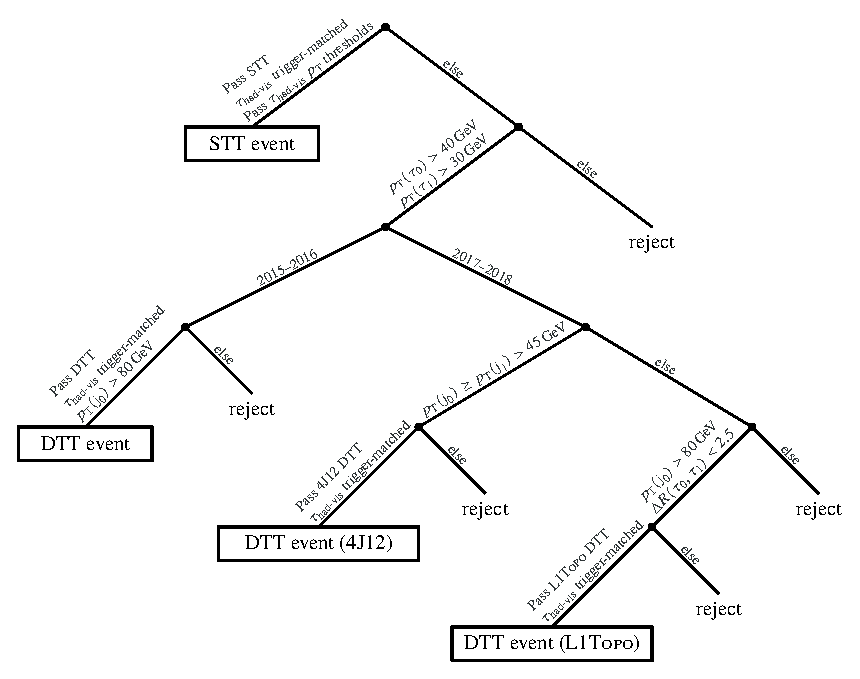
\includegraphics[width=0.95\textwidth]{selection/trigger_flowchart}

  \vspace*{0.1em}

  \caption[Flowchart of the \hadhad channel trigger selection.]{Flowchart of the
    \hadhad channel trigger selection. The leading and sub-leading \tauhadvis
    candidate (jet) from the offline event reconstruction are abbreviated as
    $\tau_0$ and $\tau_1$ ($\text{j}_0$ and $\text{j}_1$), respectively.}%
  \label{fig:trigger_selection_flowchart}
\end{figure}

The signal selection efficiency of the trigger selection varies with the
considered signal hypothesis. After an event
pre-selection,\footnote{Electron/muon veto and a \tauhadvis candidate
  pre-selection. Details are given in \Cref{tab:cutflow} of
  \Cref{sec:sr_and_cr_selection}.} the probability of an event to be selected by
the trigger, to pass the trigger-matching requirement, and to pass the
trigger-dependent \tauhadvis~\pT thresholds is about \SI{40}{\percent} for the
SM~\HH signal. For resonant production of Higgs boson pairs, the efficiency
ranges from \SI{30}{\percent} for $\mX = \SI{300}{\GeV}$ up to \SI{75}{\percent}
for $\mX = \SI{1600}{\GeV}$.

% The signal selection efficiency of offline requirements on transverse momenta
% of jets and \dRtautau range from \SI{80}{\percent} up to \SI{98}{\percent} for
% SM \HH production and resonant production for intermediate to high \mX. These
% requirements are more limiting for low \mX, e.g.\ at $\mX = \SI{300}{\GeV}$
% the efficiency is reduced to about \SI{56}{\percent}.

% STT selects only few events, predominately targeting regions of high resonance
% mass / high mHH.

% Possible plots to add: J25 turn-on???  dRtautau for L1Topo turn-on???  J12
% turn-on???


\subsection{Signal Region Event Selection}%
\label{sec:sr_and_cr_selection}

Events passing the electron, muon, \tauhadvis, and jet selections
(cf.~\Cref{tab:event_selection}) as well as the trigger selection are used to
define the SRs. Only regions with exactly two \btagged jets (2 $b$-tag regions)
are considered as SRs. Regions with fewer \btagged jets are dominated by
background processes and thus would not improve the signal sensitivity
significantly. Instead, 0 and 1 $b$-tag regions are used as control and
validation regions.

The electric charge of the electron, muon, or \tauhadvis candidate has to be
reconstructed with opposite sign (OS) with respect to the charge of the other
\tauhadvis candidate in the event. Events from processes producing \tauleptonC
pairs, such as the signal processes, \Zjets, $H \to \tautau$, and \ttbar, are
expected to be reconstructed with OS electric charge. Events with same-sign (SS)
electric charge of the visible \tauleptonC decay products predominately originate
from events in which a quark- or gluon-initiated jet is misidentified as a
\tauhadvis. Therefore, the SS region is used in the \hadhad channel for the
estimation of multi-jet backgrounds.

All events considered in this search are required to successfully pass the
di-$\tau$ mass reconstruction using the MMC. Drell--Yan processes producing
\tauleptonC pairs with low invariant mass are rejected by requiring
$\mMMC > \SI{60}{\GeV}$. In addition, the SRs of the \lephad SLT and LTT channel
only consider events fulfilling $\mBB < \SI{150}{\GeV}$. This selection allows
defining an orthogonal \ttbar CR by inverting the selection on \mBB. This region
is used for measurements related to the \faketauhadvisC background estimation.

The expected event yields after the SR selection in all three channels are
summarised in~\Cref{tab:smhh_prefit_yields}. The bulk of events entering the SRs
are from top-quark backgrounds (\ttbar and single-$t$), \Zjets, and backgrounds
in which a quark- or gluon-initiated jet is reconstructed as a \tauhadvis
($\text{jet} \to \faketauhadvis$).


\begin{table}[htbp]
  \centering

  \caption[Event yields in the SRs prior to the fit.]{Event yields in the SRs
    prior to the fit. The expected yields are shown including all statistical
    and systematic uncertainties. The SM~\HH event yields are given for the SM
    expectation. The \faketauhadvisC background estimation technique employed in
    the \lephad channels does not distinguish between different sources of
    \faketauhadvis. The category ``other backgrounds'' combines minor
    contributions from $Z \to \tautau + (bl,cl,ll)$, $Z \to e^{+}e^{-}$,
    $Z \to \mu^{+}\mu^{-}$, \Wjets, diboson and $\ttbar V$. The background
    estimation and systematic uncertainties are discussed in detail
    in~\Cref{sec:background_estimation,sec:uncertainties}.}%
  \label{tab:smhh_prefit_yields}%
  \label{tab:hadhad_presel_yields}

  \resizebox{\textwidth}{!}{
    \begin{tabular}{l
  @{\hskip 20pt}
  S[table-format=4.3(4)]
  @{\hskip 20pt}
  S[table-format=6.3(4)]
  @{\hskip 20pt}
  S[table-format=4.4(5)]}
  \toprule
  & \multicolumn{3}{c}{Signal region event yield} \\
  \cmidrule{2-4}
  Process                              & {\hadhad}      & {\lephad SLT}  & {\lephad LTT} \\
  \midrule
  SM \HH (ggF)                         & 5.4 +- 1.1     & 5.9 +- 1.2     & 1.42 +- 0.29 \\
  SM \HH (VBF)                         & 0.167 +- 0.022 & 0.200 +- 0.027 & 0.0547 +- 0.0066 \\
  SM \HH (ggF + VBF)                   & 5.6 +- 1.1     & 6.1 +- 1.2     & 1.47 +- 0.29 \\
  \midrule
  Top quark                            & 3850 +- 330    & 65300 +- 5600  & 4400 +- 460 \\
  $Z \to \tautau + (bb,bc,cc)$         & 1200 +- 210    & 1210 +- 130    & 406 +- 67 \\
  Single Higgs boson                   & 74 +- 15       & 154 +- 20      & 24.4 +- 5.0 \\
  Jet $\to \faketauhadvis$ (combined)  & {--}           & 33900 +- 6500  & 1750 +- 510 \\
  Jet $\to \faketauhadvis$ (multi-jet) & 1350 +- 150    & {--}           & {--} \\
  Jet $\to \faketauhadvis$ (\ttbar)    & 2490 +- 330    & {--}           & {--} \\
  Other backgrounds                    & 228 +- 42      & 1090 +- 210    & 119 +- 21 \\
  \midrule
  Total background                     & 9200 +- 640    & 101700 +- 8600 & 6700 +- 700 \\
  \midrule
  Observed data                        & 8380           & 98456          & 6351 \\
  \bottomrule
\end{tabular}

%%% Local Variables:
%%% mode: latex
%%% TeX-master: "../phd_thesis"
%%% End:

  }
\end{table}

The acceptance times efficiency (\AccTimesEff) for SM~\HH events in the SRs is
summarised in~\Cref{tab:nonres_acc_times_eff} for all three channels. Compared
to the previously published result in this
channel~\cite{HIGG-2016-16-witherratum}, this analysis shows an increase in the
\AccTimesEff for SM~\HH events by a factor of about 2 (1.5) for the \hadhad
(\lephad) channel. This increase is a consequence of improved \tauhadvis
reconstruction techniques and loosened identification requirements for
\tauhadvis and \btagged jets.
% compared to the previous result.
The reason for loosening the identification criteria is twofold: First, the
\tauhadvis identification and $b$-tagging algorithms were significantly
improved~\cite{ATL-PHYS-PUB-2019-033,FTAG-2019-07}, yielding reduced mistag
rates at working points with tagging efficiencies similar to the working points
used previously. Consequently, the identification criteria can be loosened while
maintaining background rates similar to the ones of the previous analysis.
Second, Higgs boson pair production has distinct kinematic features that can be
used to distinguish signal events and events containing jets that are
misidentified as $b$-jets or \tauhadvis, for example, using multivariate
methods. When exploiting these features, the signal sensitivity of this analysis
improves with a less stringent object selection.

% when exploiting the distinct kinematic features of Higgs boson pair production
% to isolate events of interest (e.g.\ using multivariate methods), then the
% sensitivity of this search is expected to be limited by statistical
% uncertainties. A looser object selection can thus serve to improve the signal
% sensitivity, provided the increase in rate of backgrounds arising from events
% with mistagged objects remains under control.

\begin{table}[htbp]
  \centering

  \caption[Acceptance times efficiency for SM~\HH events in the SRs.]{Acceptance
    times efficiency for SM~\HH events in the SRs. The \AccTimesEff is given as
    the fraction of selected events with respect to all generated
    $pp \to \HH \to \bbbar\hadhad$ ($pp \to \HH \to \bbbar\lephad$) events in
    the \hadhad (\lephad) channel. The signal acceptance of the previous
    iteration of the $\HH \to \bbtautau$ search by the ATLAS collaboration using
    \SI{36.1}{\per\femto\barn} of \pp~collision data is shown in the last
    row. $\dagger$:~The \AccTimesEff is given for the combination of \lephad SLT
    and LTT channel.}%
  \label{tab:nonres_acc_times_eff}

  \begin{tabular}{lSSS}
  \toprule
  & \multicolumn{3}{c}{Acceptance $\times$ Efficiency / \si{\percent}} \\
  \cmidrule{2-4}
  Process &\hadhad & \lephad SLT & \lephad LTT \\
  \midrule
  SM \HH (\ggF)       & 4.1 & 4.1 & 0.99 \\
  SM \HH (VBF)        & 2.3 & 2.5 & 0.68 \\
  SM \HH (\ggF + VBF) & 4.0 & 4.0 & 0.97 \\
  \midrule
  SM \HH (\ggF, early Run~2 search~\cite{HIGG-2016-16-witherratum}) & 1.9 & \multicolumn{2}{c}{3.2$^\dagger$} \\
  \bottomrule
\end{tabular}

% hadhad:
% ggF: 4.08
% VBF: 2.27
% ggF+VBF: 3.99

% lephad SLT:
% ggF: 4.08
% VBF: 2.50
% ggF+VBF: 4.00

% lephad LTT:
% ggF: 0.99
% VBF: 0.68
% ggF+VBF: 0.97

%%% Local Variables:
%%% mode: latex
%%% TeX-master: "../phd_thesis"
%%% End:

\end{table}

The majority of the increase in the \AccTimesEff for SM~\HH events with respect
to Ref.~\cite{HIGG-2016-16-witherratum} can be explained by the following
improvements:
\begin{description}

\item[\tauhadvis track association] The introduction of a multivariate method
  for \tauhadvis track association in Ref.~\cite{duschinger}, superseding a
  cut-based method, lead to an overall improvement in the \tauhadvis selection
  efficiency due to the $\Ntracks \in \{1, 3\}$ requirement on \tauhadvis. The
  relative improvement in efficiency with respect to the cut-based method is
  \SIrange[range-units=single]{20}{30}{\percent} for 1-prong \tauhadvis in the \tauhadvis \pT range
  relevant for the SM \HH search.
  % \footnote{More than \SI{80}{\percent} of SM \HH events have a leading
  % \tauhadvis candidate with \pT less than \SI{150}{\GeV}.}
  The efficiency for 3-prong \tauhadvis remains largely unchanged for \tauhadvis
  \pT below \SI{100}{\GeV} compared to the cut-based method. However, for
  3-prong \tauhadvis with $\pT > \SI{100}{\GeV}$, the track association
  efficiency is reduced by up to \SI{10}{\percent}.

\item[\Tauid] With the introduction of the RNN-based \tauid
  (cf.~\Cref{sec:tauid}), the rejection of \tauhadvis candidates originating
  from quark- or gluon-initiated jets increased by \SIrange[range-units=single]{40}{80}{\percent}
  compared to the BDT-based algorithm. This allows for a change of the
  identification working point from the \emph{medium BDT} to the \emph{loose
    RNN} working point while maintaining similar rates of \faketauhadvisC
  backgrounds. As a result, a relative increase in \tauhadvis identification
  efficiency of about \SI{13}{\percent} (\SI{25}{\percent}) is achieved for
  1-prong (3-prong) \tauhadvis.

  Additionally, an improved algorithm to reject 1-prong \tauhadvis candidates
  originating from electrons based on a BDT discriminant ($e$-veto) is used
  in this search. This algorithm improves the tagging efficiency by
  \SIrange[range-units=single]{4}{5}{\percent} for 1-prong \tauhadvis compared to the previous
  method. No $e$-veto is applied to 3-prong \tauhadvis candidates.

  % The algorithm replaced a method using the likelihood-based electron
  % identification score of an electron candidate geometrically matched to the
  % \tauhadvis, leading to a relative improvement in the tagging efficiency of
  % \SIrange[range-units=single]{4}{5}{\percent} for 1-prong \tauhadvis. No electron veto is applied
  % to 3-prong \tauhadvis candidates.

\item[$b$-tagging] Improved $b$-tagging algorithms allow for the use of working
  points with higher $b$-jet tagging efficiency while limiting the increase in
  background due to mistagged jets. Previously, the \textsc{MV2c10}
  tagger~\cite{ATL-PHYS-PUB-2016-012} with a target efficiency of
  \SI{70}{\percent} for $b$-jets from \ttbar was used. This tagger is replaced
  by the \textsc{DL1r} tagger~\cite{FTAG-2019-07} operating at the the
  \SI{77}{\percent} efficiency working point. Consequently, a \SI{10}{\percent}
  relative improvement in $b$-jet tagging efficiency is expected.

  % A new high-level tagger (\textsc{DL1r}) based on deep
  % learning~\cite{ATL-PHYS-PUB-2017-013,guth} is adopted in this search that
  % includes an impact parameter based low-level tagger using RNN
  % (\textsc{RNNIP}) as an input~\cite{ATL-PHYS-PUB-2017-003}.

  % A comparison of the working points of the \textsc{MV2c10} and \textsc{DL1r}
  % taggers with $b$-jet tagging efficiencies from \SIrange[range-units=single]{70}{77}{\percent}
  % shows an improvement in the \emph{light}- and $c$-jet rejection of
  % \SIrange[range-units=single]{80}{100}{\percent} and \SIrange[range-units=single]{20}{40}{\percent}, respectively,
  % for the \textsc{DL1r} tagger~\cite{FTAG-2019-07}.
\end{description}
These object-level efficiency improvements compound when considering the
efficiencies at event-level
% due to the selection of two $b$-tagged jets and two (one) reconstructed and
% identified \tauhadvis in the SR of the \hadhad (\lephad) channel.
and explain the majority of the increase in \AccTimesEff for SM~\HH events with
respect to the previous search in this channel.

The \AccTimesEff of the SR selection for signals from resonant \HH production
are shown in \Cref{fig:signal_acceptance_resonant} as a function of the
resonance mass. In the \hadhad channel, the acceptance of signal events from
decays of low-mass resonances is limited by the trigger selection. The signal
acceptance increases quickly with increasing \mX, reaching a maximum of about
\SI{10}{\percent} at $\mX = \SI{1000}{\GeV}$. The \AccTimesEff decreases for
resonances with masses greater than \SI{1000}{\GeV} due to the Higgs boson decay
products becoming increasingly collimated, at which point the object
reconstruction employed in this search becomes less effective at resolving the
decay products. The $\mX > \SI{1000}{\GeV}$ regime is typically covered by
dedicated searches using specialised reconstruction techniques for highly
boosted Higgs bosons (for a search in the $\bbbar\hadhad$ final state, see for
example Ref.~\cite{HDBS-2019-22}).

\begin{figure}[htbp]
  \centering

  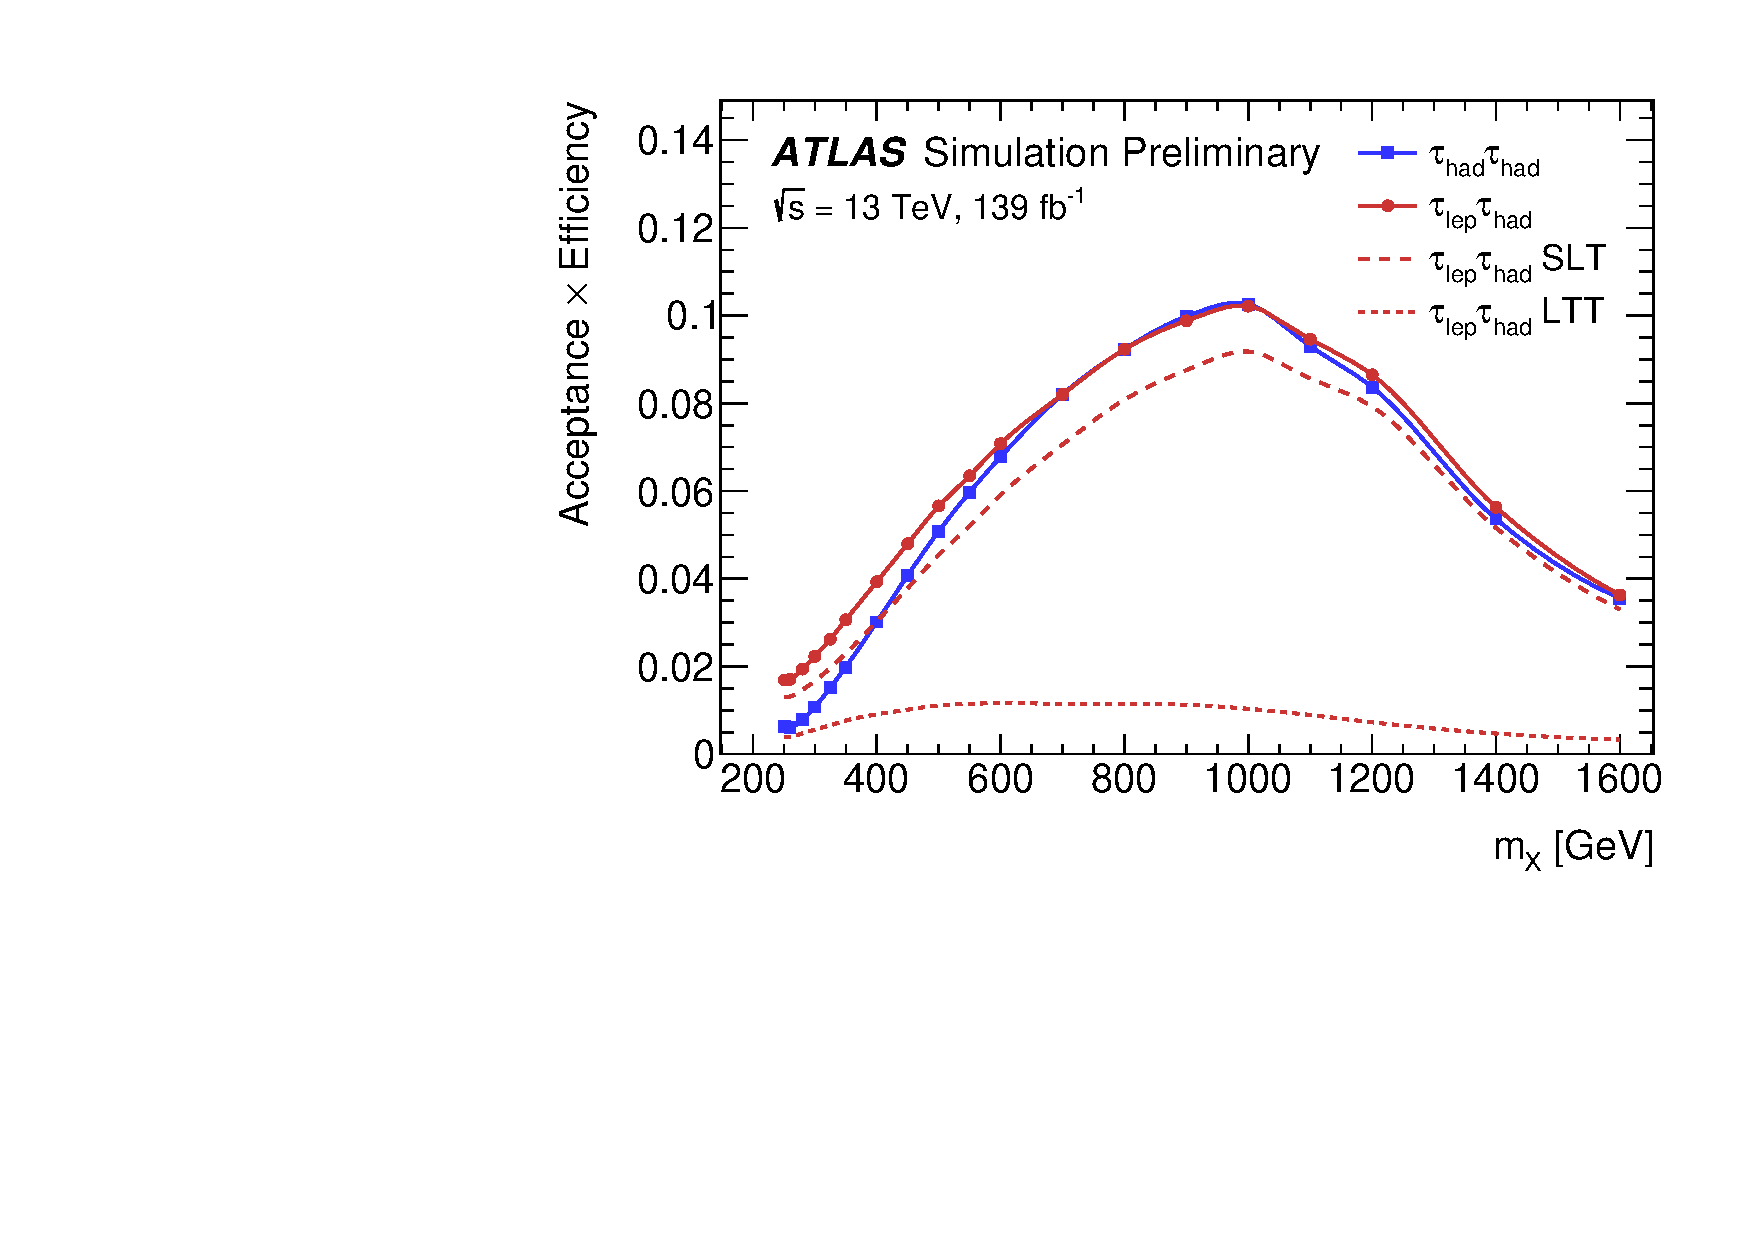
\includegraphics[width=0.6\textwidth]{selection/acceptance_resonant}

  \caption[The acceptance times efficiency of the analysis selection for events
  from scalar resonances decaying into Higgs boson pairs.]{The \AccTimesEff of
    the analysis selection for events from scalar resonances decaying into Higgs
    boson pairs. It is shown as a function of the resonance mass, \mX, and
    separately for the three channels as well as the combination of the \lephad
    SLT and LTT channel. The \AccTimesEff is given as the fraction of selected
    events with respect to all generated $\pp \to X \to \bbbar\hadhad$
    ($\pp \to X \to \bbbar\lephad$) events in the \hadhad (\lephad) channel.}%
  \label{fig:signal_acceptance_resonant}
\end{figure}

Lastly, the signal event yield after different steps of the SR event selection
of the \hadhad channel is shown in~\Cref{tab:cutflow}. Most events are lost due
to the trigger selection, the \tauhadvis candidate selection, or the requirement
of two \btagged jets in the SR.

\begin{sidewaystable}[p]
  \centering

  \caption[Event yields after different selection steps in the \hadhad channel
  for the SM~\HH signal and four exemplary signals from decays of scalar
  resonances.]{Event yields after different selection steps in the \hadhad
    channel for the SM~\HH signal and four exemplary signals from decays of
    scalar resonances. The expected number of events are normalised using the
    cross sections predicted by the SM for the SM \HH production and using
    $\sigma(pp \to X \to \HH) = \SI{10}{\femto\barn}$ for the $X \to \HH$
    signals.}%
  \label{tab:cutflow}

  \resizebox{\textwidth}{!}{
    \begin{tabular}{lS[table-format=4.1]S[table-format=3.2]S[table-format=4.2]S[table-format=4.2]S[table-format=4.1]S[table-format=4.1]}
  \toprule
  & \multicolumn{6}{c}{Expected number of events} \\
  \cmidrule{2-6}
  Selection step & {SM \HH (\ggF)} & {SM \HH (VBF)} & {$X(\SI{300}{\GeV})$} & {$X(\SI{500}{\GeV})$} & {$X(\SI{1000}{\GeV})$} & {$X(\SI{1600}{\GeV})$} \\
  \midrule
  \HH                            & 4310 & 240   & 1390 & 1390 & 1390 & 1390 \\
  $\HH \to \bbtautau$            & 315  & 17.5  & 102  & 102  & 102  & 102  \\
  $\HH \to \bbbar\tauhad\tauhad$ & 132  & 7.36  & 42.6 & 42.6 & 42.6 & 42.6 \\
  \midrule
  Generator filters              & 103  & 5.0   & 26.5 & 32.6 & 37.5 & 39.5 \\
  Derivation skim                & 88.3 & 4.24  & 21.7 & 28.4 & 33.3 & 23.6 \\
  $e$ / $\mu$ selection (veto)   & 84.4 & 4.03  & 20.9 & 27.5 & 31.8 & 22.0 \\
  Initial \tauhadvis selection   & 40.4 & 1.89  & 9.25 & 13.6 & 17.5 & 10.2 \\
  Trigger selection              & 17.3 & 0.744 & 2.79 & 6.56 & 12.4 & 7.70 \\
  2nd \tauhadvis selection       & 17.3 & 0.741 & 2.78 & 6.55 & 12.4 & 7.66 \\
  Jet selection                  & 16.0 & 0.641 & 2.52 & 6.17 & 12.1 & 7.35 \\
  \bottomrule
\end{tabular}


%%% Local Variables:
%%% mode: latex
%%% TeX-master: "../phd_thesis"
%%% End:

  }
\end{sidewaystable}

% A number of control and validation regions are used in this analysis. These
% regions are summarised in the following, a detailed description following in
% the referenced sections:
% \begin{description}

% \item[$Z \ra \ell^{+}\ell^{-}$ ($\ell = e, \mu$) CR] A control
%   region targeting the production of $Z$ bosons in association with quarks of
%   heavy flavour in a di-lepton final state and two \btagged jets. This region
%   is used for background estimation in \Cref{sec:bkg_zjets}.

% \item[\ttbar CR] CRs defined in the \lephad channel
%   by inverting the $\mBB$ selection of the SR. This region targets
%   the production of \ttbar with a final state containing $\ell + \tauhadvis$
%   and is used for the estimation of \faketauhadvisC backgrounds from \ttbar
%   production in the \hadhad~(\Cref{sec:bkg_hadhad_ttbarfakes}) and \lephad
%   channels~(\Cref{sec:bkg_lephad_combined_ff}).

% \item[Anti-ID and SS control / validation regions (\hadhad channel)] Multiple
%   control and validation regions are defined by relaxing the \tauid
%   requirements, by considering events with SS \tauhadvis candidate charges,
%   and by considering regions with 1 and 2 \btagged jets. These regions are
%   enhanced in backgrounds containing \faketauhadvis and are used for the
%   estimation of the multi-jet background in \Cref{sec:bkg_hadhad_ff}.

% \item[Multi-jet / W+jets CR? Anti-Isolation? (\lephad channels)]
%   \Cref{sec:bkg_lephad_combined_ff}

% \item[Validation regions] \todo[inline]{Put text here...}

% \end{description}


%%% Local Variables:
%%% mode: latex
%%% TeX-master: "../../phd_thesis"
%%% End:
